\documentclass[conference,onecolumn]{IEEEtran}
\IEEEoverridecommandlockouts

\usepackage{cite}
\usepackage{amsmath,amssymb}
\usepackage{graphicx}
\usepackage{textcomp}
\usepackage{xcolor}
\usepackage{booktabs}
\usepackage{tabularx}
\usepackage{array}
\usepackage{url}

\Urlmuskip=0mu plus 2mu\relax
\def\UrlBreaks{\do\/\do-\do\_\do\.\do\?\do\=\do\&}
\emergencystretch=2em
\graphicspath{{../results/presentation/}{../results/}}

\newcolumntype{Y}{>{\raggedright\arraybackslash}X}
\newcommand{\pjbit}{pJ/bit}
\newcommand{\tbps}{Tb/s}
\newcommand{\gbs}{GB/s}
\newcommand{\figref}[1]{Fig.~\ref{#1}}
\newcommand{\tabref}[1]{Table~\ref{#1}}

\def\BibTeX{{\rm B\kern-.05em{\sc i\kern-.025em b}\kern-.08em
    T\kern-.1667em\lower.7ex\hbox{E}\kern-.125emX}}

\begin{document}

\title{Photonic Interconnects for TPU-Class LLM Systems}

\author{
\IEEEauthorblockN{Pranav Sitaraman}
\IEEEauthorblockA{6.5930 Hardware Architecture for Deep Learning}
\and
\IEEEauthorblockN{Simone Surdi}
\IEEEauthorblockA{6.5930 Hardware Architecture for Deep Learning}
}

\maketitle

\section{Project Overview}

This project follows Project 12, ``Evaluate a New Technology.'' We study
Lightmatter-style co-packaged photonic interconnects as a replacement or
augmentation for electrical inter-chip interconnect in TPU-class accelerator
systems. The starting point is AccelForge, which gives us a local accelerator
mapper and memory hierarchy. We extend that setup with a network model,
a logical cluster-memory level, a distributed mapping selector, and a small
compiler/dataflow model for LLM-scale systems.

The motivating problem is simple: modern LLM training and inference are not
only matrix multiplication problems. A full system also moves activations,
KV-cache state, shared weights, expert tokens, gradients, and optimizer state
across thousands of chips. Public TPU7x/Ironwood documentation lists a
9216-chip pod, 192 GiB of HBM per chip, 7380 \gbs{} of HBM bandwidth per chip,
and 1200 \gbs{} of bidirectional ICI bandwidth per chip \cite{tpu7x}. That is
an enormous machine, but it is still a distributed memory machine.

The project asks whether photonics merely lowers the cost of those bits, or
whether it changes the way the system should be mapped. Lightmatter's public
M1000 EVK page reports 114.6 \tbps{} total bidirectional bandwidth and
2.3 \pjbit{} system efficiency including laser power \cite{m1000}. The
EVK100 material reports 1.6 \tbps{} unidirectional transmission on one fiber,
or 3.2 \tbps{} bidirectional-class service with separate transmit and receive
fibers, plus a conservative 3.2 \pjbit{} point. The broader Passage family page
also advertises a 1.9 \pjbit{} reference point \cite{evk100,passage}. Those
numbers matter, but the more interesting properties are high radix, flatter
paths, and natural multicast.

Our hypothesis is therefore narrow and testable. Optical links should help
most when communication leaves a local HBM bank or fans out to many chips.
Node-to-node exchange should improve less, because a TPU torus is already
reasonable for local traffic. Shared-state multicast, remote pooled-HBM
streaming, KV-cache movement, and MoE routing should improve more. We also
expect inference to benefit more than training: once gradient traffic is
reduced, training becomes dominated by compute and HBM.

\begin{figure}[t]
    \centering
    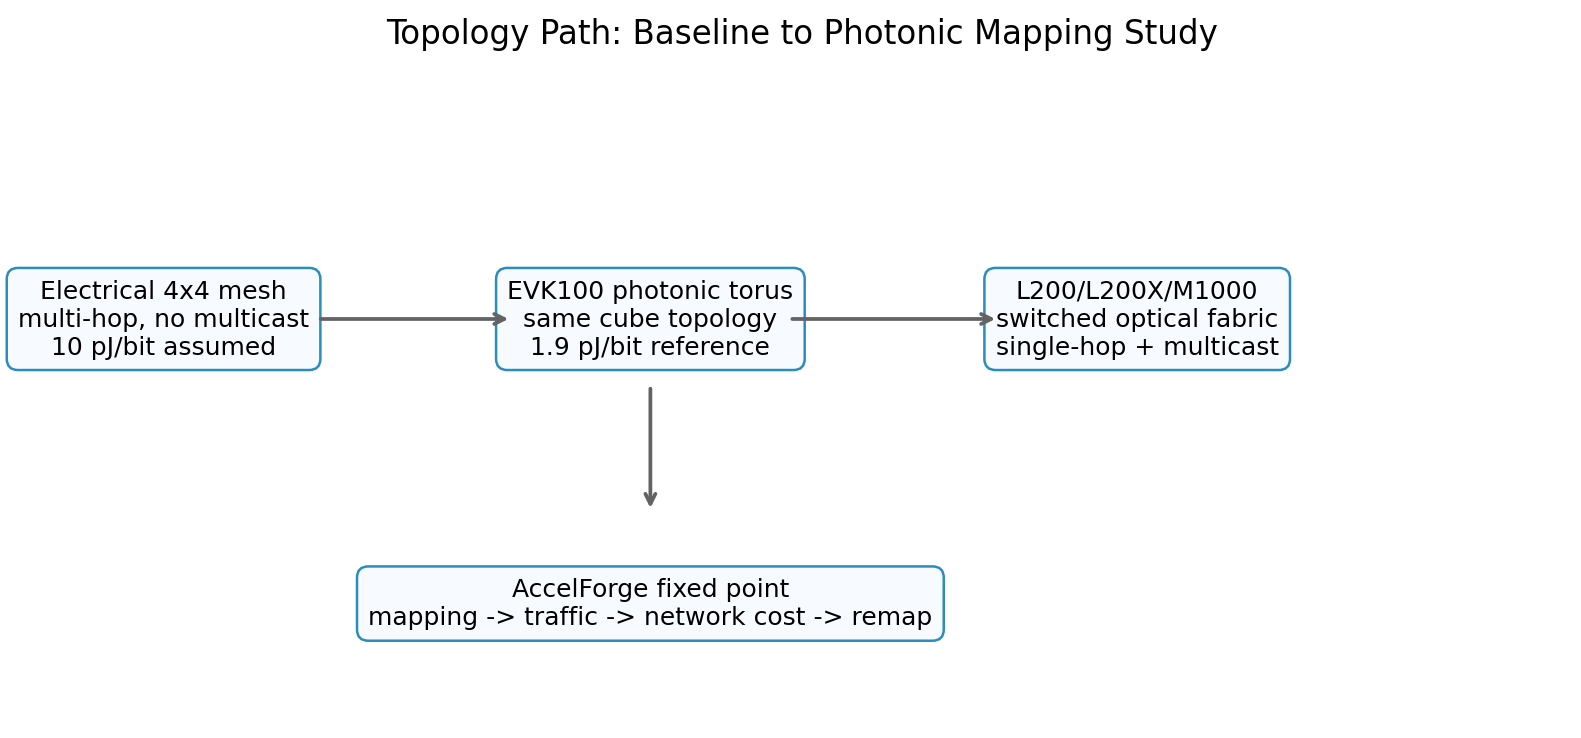
\includegraphics[width=0.72\linewidth]{03_topology_diagram.png}
    \caption{Modeling scope. AccelForge supplies local mappings and logical
    memory traffic; the project prices that traffic under electrical mesh/torus,
    advanced chiplet, photonic torus, and switched photonic fabrics.}
    \label{fig:topology}
\end{figure}

\section{Technical Contributions}

The project has four pieces.

First, we implement topology models for electrical mesh/torus networks,
advanced chiplet links, and photonic crossbar or switched fabrics. The model
does not treat the network as a single bandwidth multiplier. It includes hop
count, contention, per-hop latency, link energy, and whether multicast is
available.

Second, we integrate the network with AccelForge by adding a logical memory
level that represents the union of accelerator memories. The workflow is:
run the mapper, extract logical-memory traffic, evaluate the network cost, add
that cost back to the logical memory level, and rerun until the result
stabilizes. This gives the mapper a chance to react to network-aware memory
costs rather than treating remote memory as free.

Third, we add a distributed mapping selector. It compares node-to-node
activation exchange, node-to-DRAM remote fetch, and shared-DRAM multicast.
This is where we can see if a photonic fabric changes the best communication
pattern, even when the inner GEMM tile mapping remains conservative.

Fourth, we add a compiler/dataflow layer above AccelForge. This layer is meant
to resemble the choices a TPU software stack would expose: XLA/GSPMD-style
collectives, software-managed cache fills, remote pooled-HBM streaming,
photonic multicast prefetch, and MoE locality routing. PyTorch/XLA describes
GSPMD as a system where the compiler partitions a single-device program using
sharding hints and inserts the necessary collectives \cite{xla}. Our model asks
how those hints should change when multicast and remote memory become cheaper.

\begin{table}[t]
\centering
\caption{Main assumptions used in the proposal. Values come from public
documentation or from the explicit project baseline.}
\label{tab:assumptions}
\footnotesize
\begin{tabularx}{\linewidth}{lY}
\toprule
Item & Assumption \\
\midrule
TPU system & TPU7x/Ironwood full pod: 9216 chips, 192 GiB HBM/chip, 1200 \gbs{} bidirectional ICI/chip \cite{tpu7x}. \\
Electrical baseline & TPU-like torus with 800 Gb/s directional links and 10 \pjbit{} link energy in the AccelForge-scale study. \\
Advanced chiplet baseline & Prompt-specified comparison point: 3.5 \tbps{} one-way bandwidth and 6 \pjbit{} per network hop. \\
EVK100 photonic point & 1.6 \tbps{} unidirectional fiber point, or 3.2 \tbps{} bidirectional-class service with separate transmit and receive fibers; 3.2 \pjbit{} conservative EVK value and 1.9 \pjbit{} Passage-family optimistic reference \cite{evk100,passage}. \\
M1000 photonic point & 114.6 \tbps{} total bidirectional bandwidth and 2.3 \pjbit{} including laser power \cite{m1000}. \\
Gemini-class workload & Public dense, MoE, and long-context proxies. We do not claim Google has published Gemini 3/3.1 parameter counts. \\
\bottomrule
\end{tabularx}
\end{table}

The main tradeoff is that this is an architecture model, not a packet-level
network simulator. It captures the effects most relevant to mapping and
accelerator design, but it does not model queueing transients, virtual-channel
details, or optical-switch reconfiguration timing. That is acceptable for this
project because the goal is to decide where the new technology changes the
architecture, not to reproduce a vendor switch microarchitecture.

\section{Evaluation}

The evaluation keeps the local accelerator compute and HBM hierarchy fixed
unless a specific experiment says otherwise. The baseline is an electrical
TPU-like fabric. The proposed systems are EVK100-style photonic torus/crossbar
models and M1000-style switched optical fabrics. We also include the stronger
advanced chiplet baseline so the comparison is not artificially easy.

\begin{table}[t]
\centering
\caption{Pilot results already produced by the project pipeline. These are the
numbers the final experiments will explain rather than just report.}
\label{tab:pilot}
\footnotesize
\begin{tabularx}{\linewidth}{l r Y}
\toprule
Result & Value & What it suggests \\
\midrule
16-node AccelForge energy reduction & 72.21\% & Optical multicast helps most when shared state fans out to many nodes. \\
16-node AccelForge latency reduction & 97.57\% & Remote/shared traffic can dominate exposed latency under the electrical mesh. \\
TPU cube M1000 multicast energy reduction & 99.91\% & A switched optical fabric avoids repeated torus fanout for shared weights. \\
Distributed mapping changes & 5 of 16 cases & Photonics can make shared-DRAM multicast preferable to node-to-node exchange. \\
Compiler/dataflow energy gain & 67.75\% & Remote pooled-HBM streaming becomes attractive on M1000 for KV attention. \\
Full-pod inference speedup & 14.50$\times$ & Long-context proxy inference is highly network exposed. \\
Full-pod training speedup & 1.43$\times$ & Training improves, but becomes compute/HBM dominated after collectives shrink. \\
\bottomrule
\end{tabularx}
\end{table}

\subsection{Experiment 1: AccelForge mapping with network feedback}

We will run LLM-shaped kernels such as decode MLP, KV attention, prefill
projection, MoE dispatch, and training weight-gradient accumulation on a
16-node cluster and a 4 by 4 by 4 TPU cube. For each workload, we compare
node-to-node exchange, node-to-DRAM fetch, and shared-DRAM multicast.

The metrics are total energy, total latency, network energy share, and whether
the fixed-point mapping or distributed mapping choice changes. The expected
trend is that node-to-node traffic changes least, while remote weight/KV fetch
and shared multicast change most. This directly tests the class idea that data
movement dominates when reuse is poor or when state is replicated through a
memory hierarchy.

\subsection{Experiment 2: topology, scaling, and the chiplet baseline}

The second experiment sweeps from one 64-chip cube toward 9216 chips. We will
compare electrical torus, advanced chiplet torus, EVK100 photonic torus, and
M1000 switched optical fabric. The key output is a scaling plot with per-chip
energy or latency on the y-axis and chip count on the x-axis.

The expected result is not that every optical link wins everywhere. A photonic
torus still inherits torus hop growth. The stronger claim is that switched
photonics changes the scaling law for global traffic by flattening logical
distance and making multicast closer to one transfer than to many unicasts.

\subsection{Experiment 3: compiler-visible LLM dataflow}

The third experiment moves above the local mapper. We model whether a compiler
should prefer classic XLA/GSPMD collectives, replicated cache fills, remote
pooled-HBM streaming, photonic multicast prefetch, or MoE locality routing.
This matters because the AccelForge tile mapping can stay the same while the
best system-level dataflow changes.

\begin{figure}[t]
    \centering
    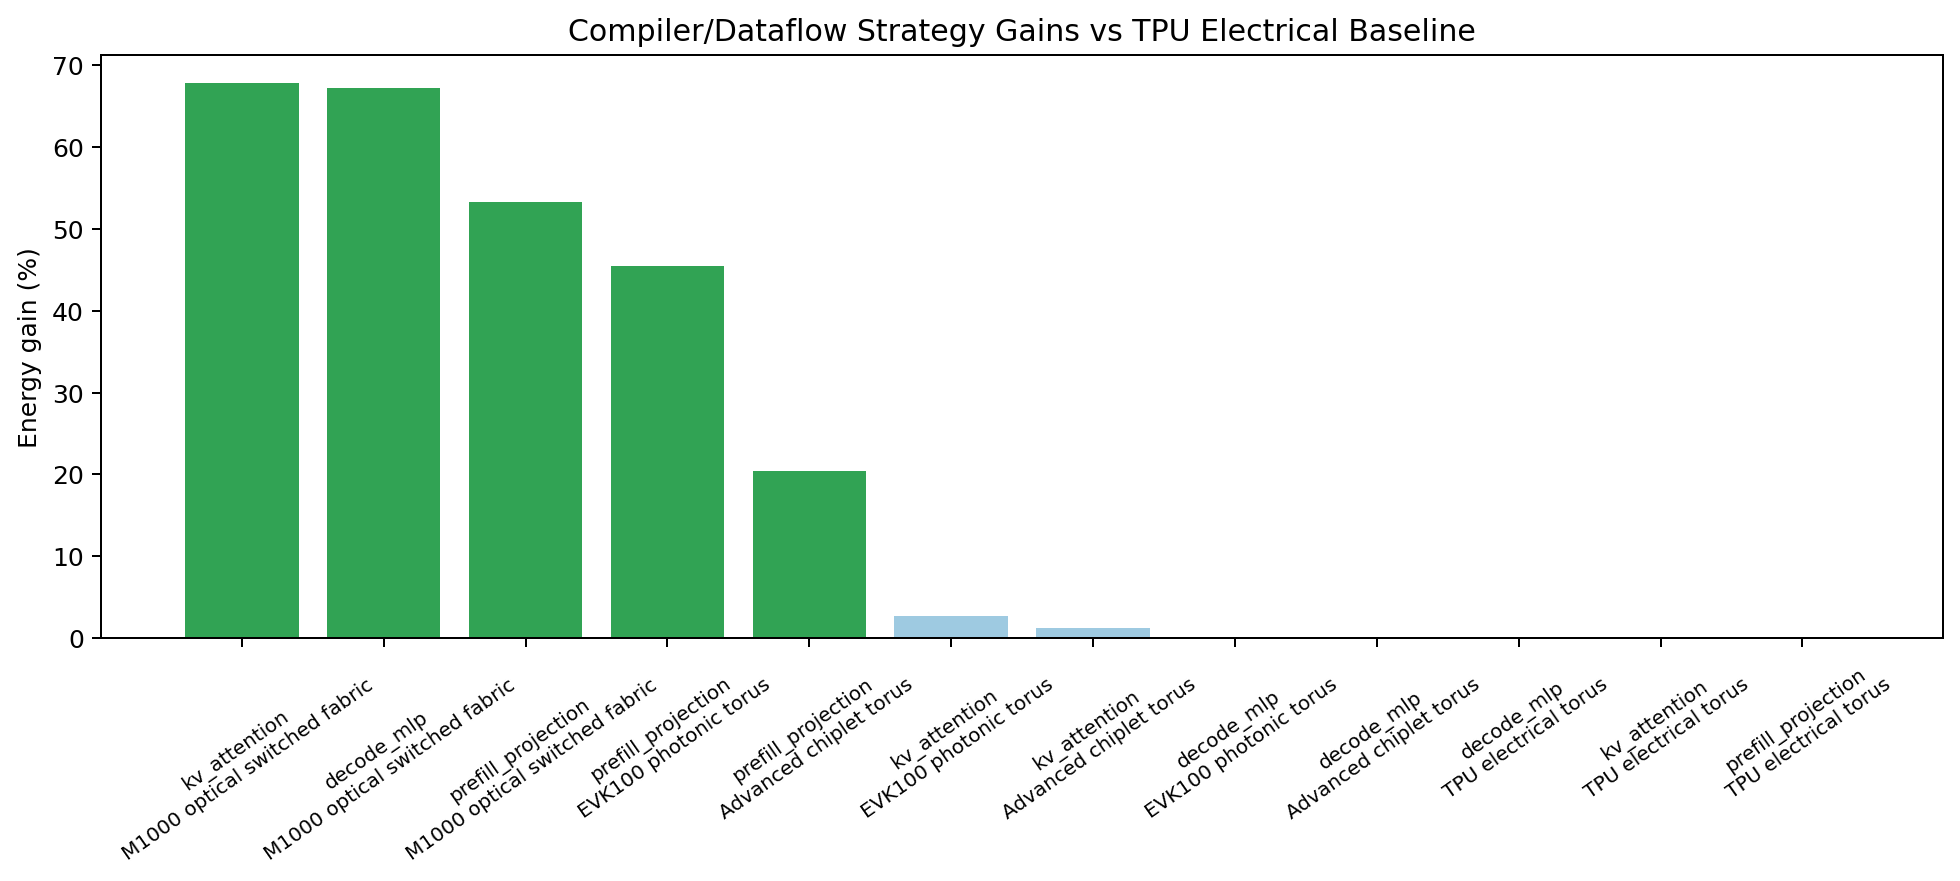
\includegraphics[width=0.70\linewidth]{04_compiler_strategy_choices.png}
    \caption{Compiler/dataflow pilot result. The important change is not in
    every local tile; it is in the choice between collectives, remote pooled HBM,
    and multicast cache fills.}
    \label{fig:compiler}
\end{figure}

The full-system version of this experiment uses a 9216-chip Ironwood pod and
Gemini-class proxy workloads: a dense Flash-like proxy, a sparse MoE Pro-like
proxy, and a long-context Deep Think-like proxy. We separate inference into
prefill, decode KV attention, weight/expert refill, and MoE dispatch. We
separate training into forward/backward compute, gradient synchronization,
training MoE dispatch, and optimizer-state traffic.

\begin{figure}[t]
    \centering
    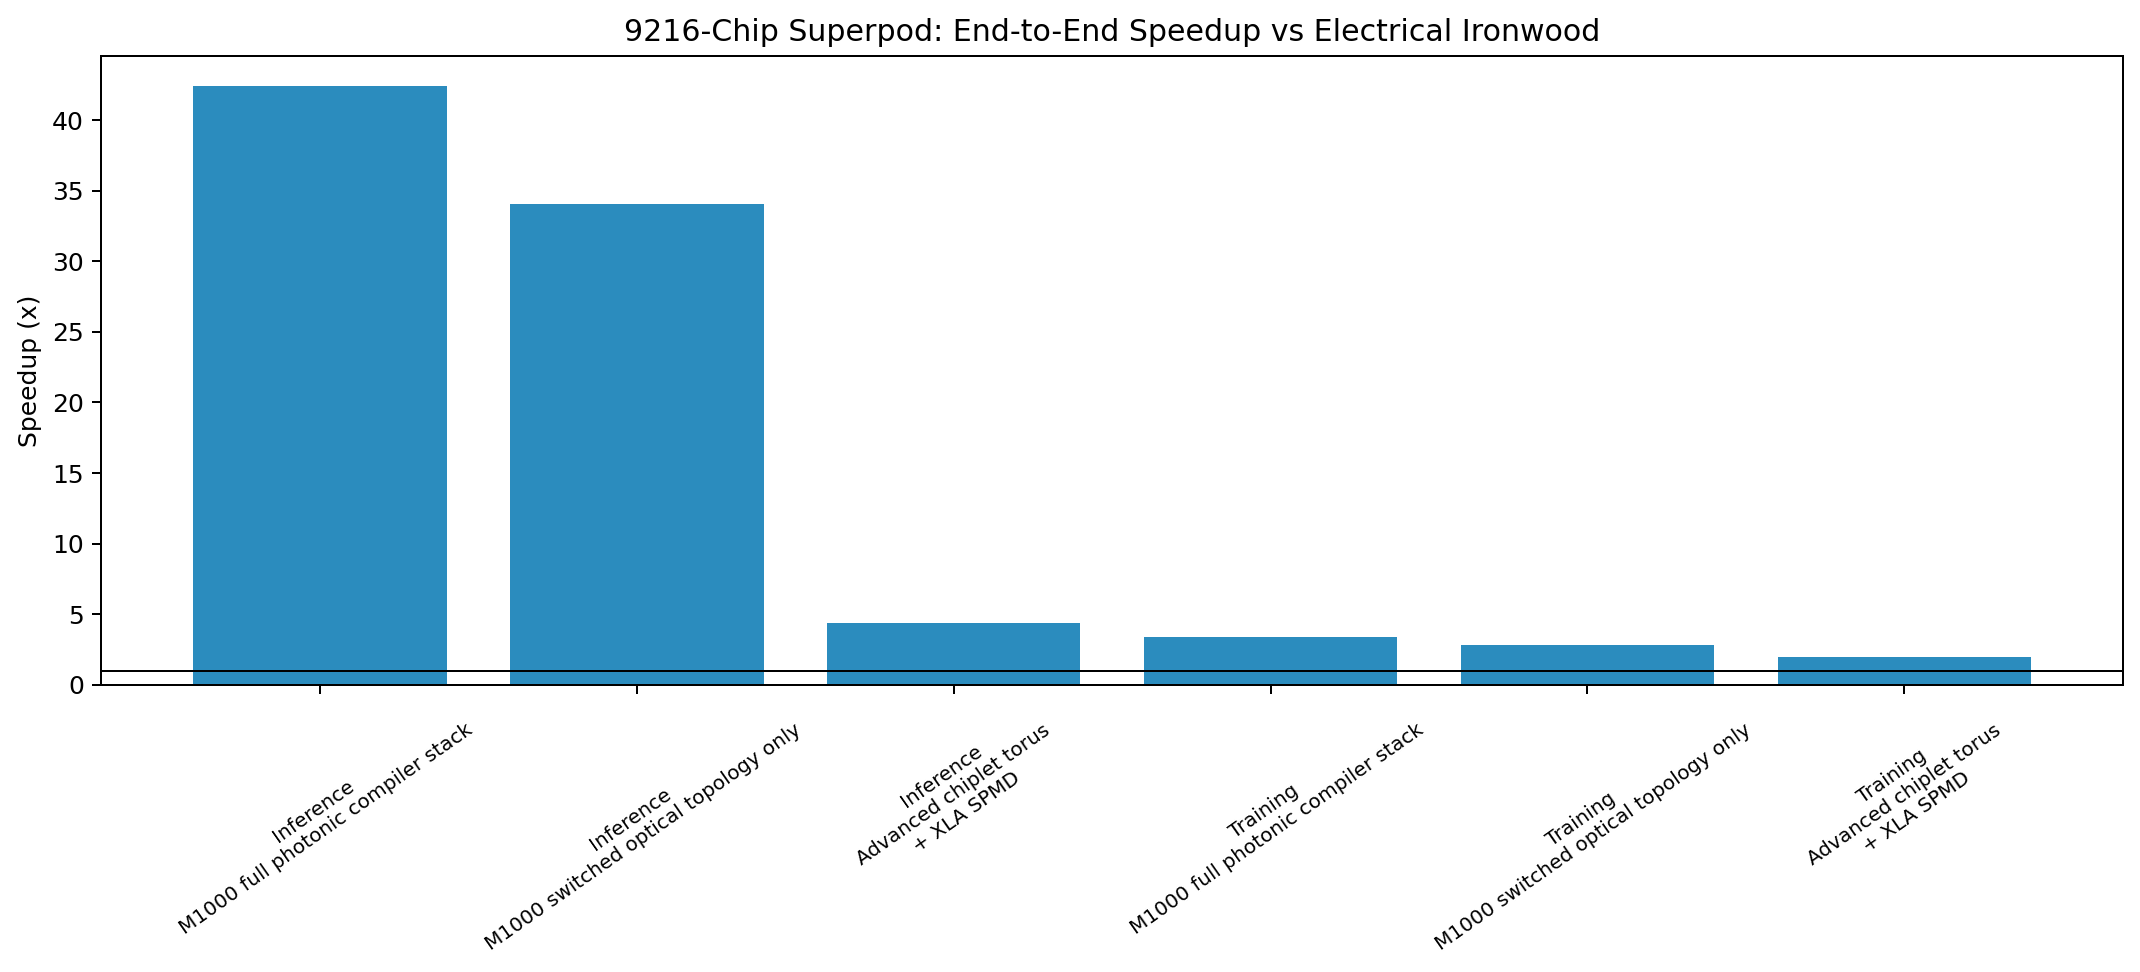
\includegraphics[width=0.70\linewidth]{07_superpod_end_to_end_speedups.png}
    \caption{End-to-end superpod pilot result. The model predicts much larger
    gains for inference than for training because inference leaves more network
    latency exposed after compute/HBM overlap.}
    \label{fig:superpod}
\end{figure}

\begin{figure}[t]
    \centering
    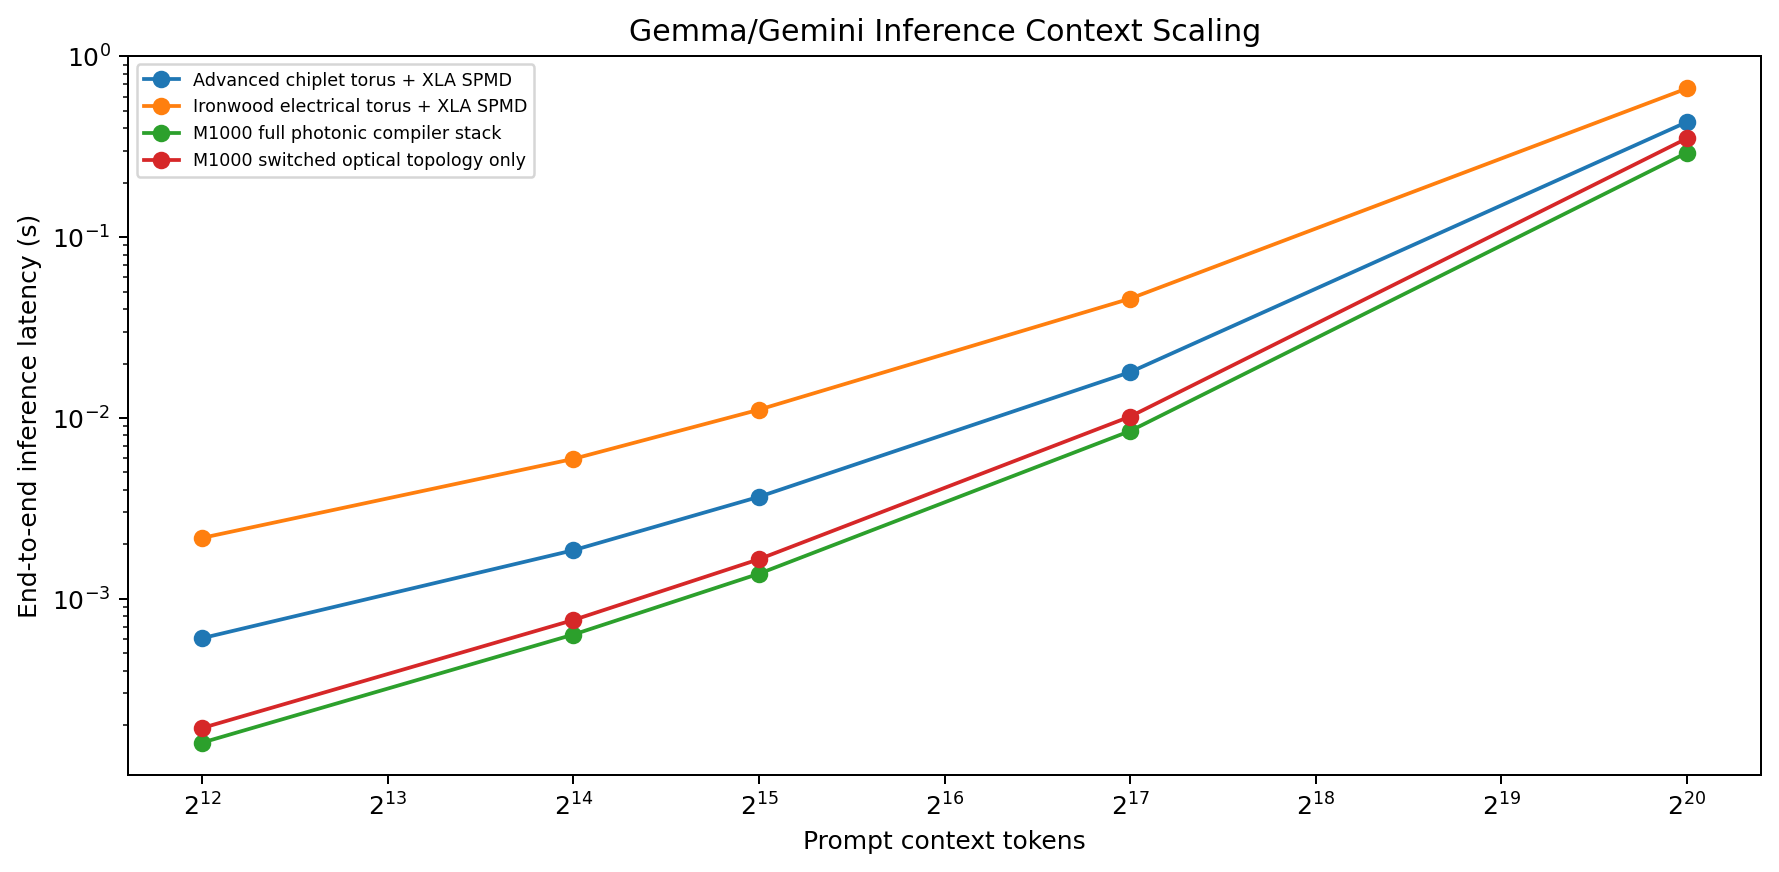
\includegraphics[width=0.70\linewidth]{09_superpod_context_scaling.png}
    \caption{Context-length pilot result. Long-context inference is the case
    where better multicast, remote memory, and flatter topology are expected to
    matter most.}
    \label{fig:context}
\end{figure}

The final output will be an ablation ladder: electrical baseline, advanced
chiplet, photonic torus with multicast, switched topology, multicast cache,
remote pooled HBM, MoE locality routing, and full photonic compiler stack. This
will make the answer less hand-wavy. We can say which part of the improvement
comes from better links, which part comes from topology, and which part comes
from changing the compiler-visible dataflow.

\section{Timeline and Work Distribution}

The modeling code is already in place, and the remaining work is mostly
validation, polish, and interpretation. Simone will focus on the AccelForge
network loop, topology model, and mapping-level validation. Pranav will focus
on the compiler/dataflow model, superpod study, figures, and final writeup.
Both of us will review the final assumptions and presentation.

\begin{table}[t]
\centering
\caption{Project plan from the current state to submission.}
\label{tab:timeline}
\footnotesize
\begin{tabularx}{\linewidth}{lY}
\toprule
Step & Deliverable \\
\midrule
Topology and logical memory & Complete the network model, logical memory level, and fixed-point AccelForge loop. \\
Mapping study & Report node-to-node, node-to-DRAM, and shared-multicast results with mapping-change counts. \\
Scaling and baselines & Compare electrical TPU, advanced chiplet, EVK100, and M1000 from cube scale to superpod scale. \\
Compiler/dataflow study & Explain when XLA-style collectives give way to multicast cache fills or remote pooled HBM. \\
Final synthesis & Produce a short paper, notebook, and slide deck with the same assumptions, figures, and headline numbers. \\
\bottomrule
\end{tabularx}
\end{table}

The main risk is overclaiming. We will keep the final paper explicit about what
is measured in AccelForge, what is modeled analytically, and what is based on
public proxy workloads. That boundary is also what makes the project useful:
it shows where photonic interconnects change the accelerator design problem
without pretending to know private TPU or Gemini implementation details.

\begin{thebibliography}{99}

\bibitem{tpu7x}
Google Cloud, ``TPU7x (Ironwood),'' viewed Apr. 2026.
\url{https://docs.cloud.google.com/tpu/docs/tpu7x}

\bibitem{m1000}
Lightmatter, ``Passage M1000 EVK,'' viewed Apr. 2026.
\url{https://lightmatter.co/products/passage-m1000-evk/}

\bibitem{evk100}
Lightmatter, ``Passage EVK100,'' viewed Apr. 2026.
\url{https://lightmatter.co/products/passage-evk100/}

\bibitem{passage}
Lightmatter, ``Passage product family,'' viewed Apr. 2026.
\url{https://lightmatter.co/products/passage}

\bibitem{xla}
PyTorch/XLA, ``SPMD user guide,'' viewed Apr. 2026.
\url{https://docs.pytorch.org/xla/master/spmd.html}

\end{thebibliography}

\end{document}
